\documentclass[12pt, a4paper]{article}

\usepackage{amsmath}
\usepackage{array}
\usepackage{amsmath}
\usepackage[portuguese]{babel}
\usepackage{chngpage}
\usepackage{float}
\usepackage[a4paper, margin=2cm]{geometry}
\usepackage{graphicx}
\usepackage{hyperref}
\usepackage{listings}
\usepackage{setspace}
\usepackage{xcolor}

\lstdefinestyle{codestyle}{
    commentstyle=\color{teal},
    keywordstyle=\color{blue},
    numberstyle=\ttfamily\color{gray},
    stringstyle=\color{red},
    basicstyle=\ttfamily\footnotesize,
    breakatwhitespace=false,
    breaklines=false,
    keepspaces=true,
    numbers=none,
    showspaces=false,
    showstringspaces=false,
    showtabs=false,
    tabsize=4
}
\lstset{style=codestyle}

\title{\Huge \textbf{Computação Gráfica \\ \Large Trabalho Prático -- Fase II}}
\date{30 de março 2025}
\author{Grupo 3}

\begin{document}

\begin{center}
    
\includegraphics[width=0.25\textwidth]{res/cover/EE-C.eps}
\end{center}

\chardef\_=`_
\onehalfspacing
\setlength{\parskip}{\baselineskip}
\setlength{\parindent}{0pt}
\def\arraystretch{1.5}

{\let\newpage\relax\maketitle}
\maketitle
\thispagestyle{empty}

\vspace*{\fill}

\begin{adjustwidth}{-2cm}{-2cm} % These values only need to be large enough to center the table
    \begin{center}
        \begin{tabular}{>{\centering}p{0.25\textwidth}
                        >{\centering}p{0.25\textwidth}
                        >{\centering}p{0.25\textwidth}
                        >{\centering\arraybackslash}p{0.25\textwidth}}
            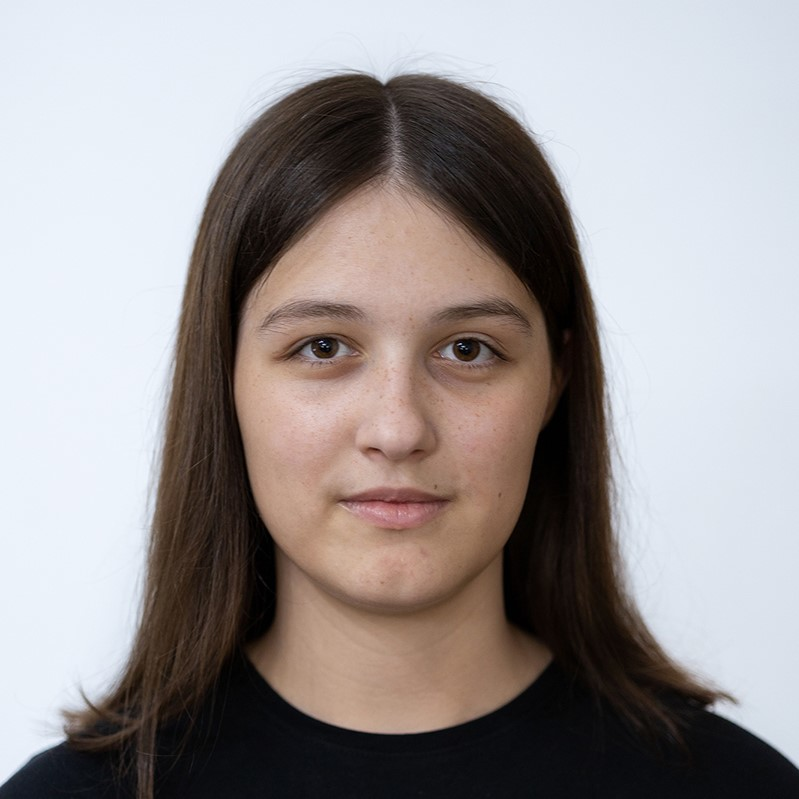
\includegraphics[width=3.5cm]{res/cover/A104437.png} &
            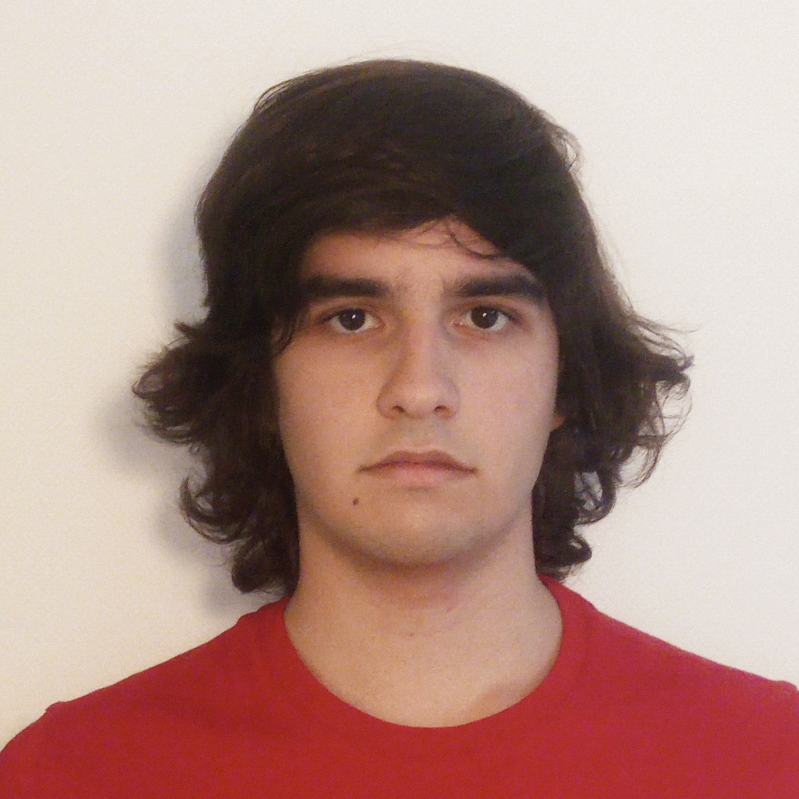
\includegraphics[width=3.5cm]{res/cover/A104348.png} &
            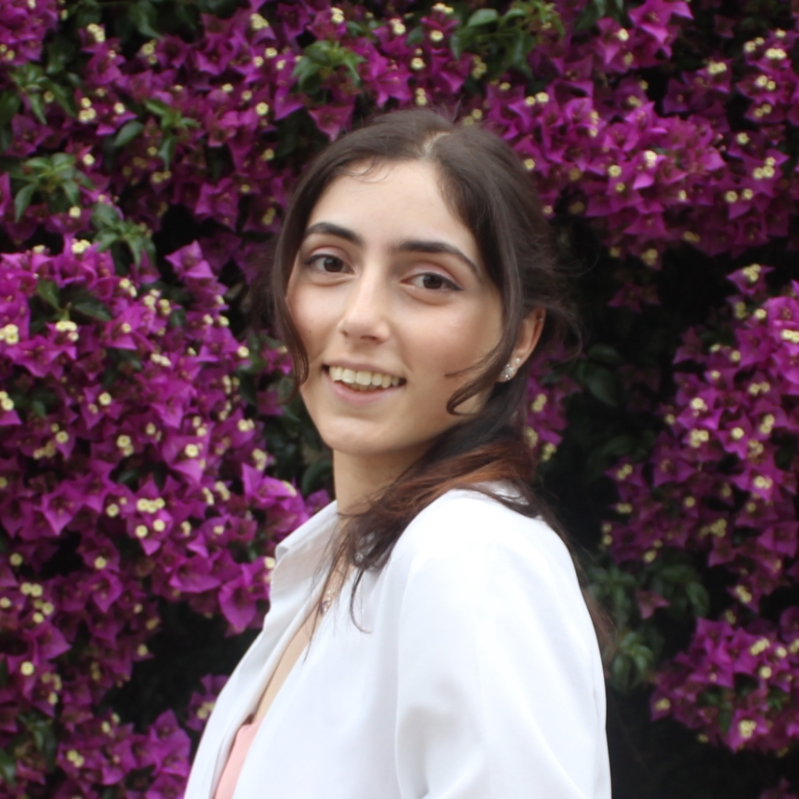
\includegraphics[width=3.5cm]{res/cover/A90817.png} &
            
\includegraphics[width=3.5cm]{res/cover/A104179.png} \\

            Ana Oliveira & Humberto Gomes & Mariana Cristino & Sara Lopes \\
            A104437      & A104348        & A90817           & A104179
        \end{tabular}
    \end{center}
\end{adjustwidth}

\pagebreak

\begin{abstract}
    \textbf{\color{red} TODO - resumo}
\end{abstract}

\section{Transformações}

\textbf{\color{red} TODO - transformações}

\section{Sistema Solar Estático}

\subsection{Hierarquia do Sistema Solar}

O sistema solar foi representado através de uma estrutura hierárquica que segue a disposição
real
dos corpos celestes. No nível mais elevado encontra-se o Sol, que serve de ponto central e de
referência para a órbita dos restantes corpos celestes.

Cada planeta foi colocado num grupo independente, associado diretamente ao Sol. Quando aplicável,
os satélites naturais (luas) e os aneis são inseridos como grupos filhos do planeta
correspondente, preservando a hierarquia entre os corpos. A cintura de asteróides, por sua vez,
é representada como um grupo filho do Sol, uma vez que orbita em torno deste.

Desta forma, assegura-se que:
\begin{itemize}
    \item os planetas orbitam em torno do Sol;
    \item as luas orbitam em torno do planeta a que pertencem;
    \item os anéis acompanham o planeta respetivo;
    \item os asteróides se posicionam nas suas cinturas, em órbitas relativas ao Sol.
\end{itemize}

\subsection{Representação em XML}

A estrutura em XML segue a hierarquia descrita anteriormente. Cada grupo define transformações
aplicadas aos seus elementos, como \texttt{translate}, \texttt{rotate} e \texttt{scale}, que são
acumuladas ao longo da árvore de grupos. Esta organização permite simular corretamente os
movimentos
e proporções relativos entre os corpos celestes, como as órbitas dos planetas em torno do Sol
ou
das luas em torno dos seus planetas.

Abaixo apresenta-se um exemplo com o Sol, a Terra e a Lua:

\begin{lstlisting}
<group>
    <!-- Grupo do sol -->
    <group>
        <transform>
            <translate x="0" y="0" z="0"/>
            <scale x="30" y="30" z="30"/>
        </transform>
        <models>
            <model file="../models/sphere.3d"/>
        </models>
        <!-- Grupo do planeta Terra -->
        <group>
            <transform>
                <translate x="28" y="0" z="-3"/>
                <scale x="0.2" y="0.2" z="0.2"/>
            </transform>
            <models>
                <model file="../models/sphere.3d"/>
            </models>
            <!-- Grupo da lua -->
            <group>
                <transform>
                    <translate x="3" y="0" z="0"/>
                    <scale x="0.05" y="0.05" z="0.05"/>
                </transform>
                <models>
                    <model file="../models/sphere.3d"/>
                </models>
            </group>
        </group>
    </group>
</group>
\end{lstlisting}

Neste exemplo:
\begin{itemize}
    \item O primeiro \texttt{group} representa o Sol, posicionado na origem e aumentado com
    \texttt{scale}.
    \item Dentro do grupo do Sol encontra-se a Terra, posicionada com \texttt{translate} e
    redimensionada.
    \item Dentro do grupo da Terra está a Lua, com a sua própria transformação relativa.
\end{itemize}

As transformações são aplicadas sequencialmente e propagam-se ao longo da hierarquia. Assim, a
posição e a escala de cada corpo são relativas ao seu elemento pai, respeitando a estrutura do
sistema solar. Isto permite gerar movimentos orbitais e tamanhos proporcionais com base em
operações simples.

Além dos planetas e das luas, existem dois tipos de elementos adicionais com representação
específica no XML:

\begin{itemize}
    \item As \textbf{cinturas de asteróides} são compostas por figuras \texttt{sphere.3d},
    \texttt{box.3d} e \texttt{cylinder.3d}, escolhidas aleatoriamente. Estas instâncias são
    adicionadas como grupo filho do Sol e posicionadas com coordenadas aleatórias em torno de um
    raio definido. Cada asteróide recebe transformações próprias de \texttt{translate},
    \texttt{rotate} e \texttt{scale}, simulando a sua dispersão e dimensão variável.

    \item Os \textbf{anéis} reutilizam o modelo \texttt{torus.3d} da Fase I. Para
    simular a sua aparência achatada, é aplicada uma \texttt{scale} com fator reduzido no eixo
Y.
    Além disso, os anéis são orientados através de uma rotação (\texttt{rotate}) com
ângulo e
    eixo ajustados consoante o planeta. Cada anel é inserido como grupo filho do planeta
    correspondente.
\end{itemize}

O resultado destas pode ser visto na seguinte figura:

\begin{figure}[H]
    \centering
    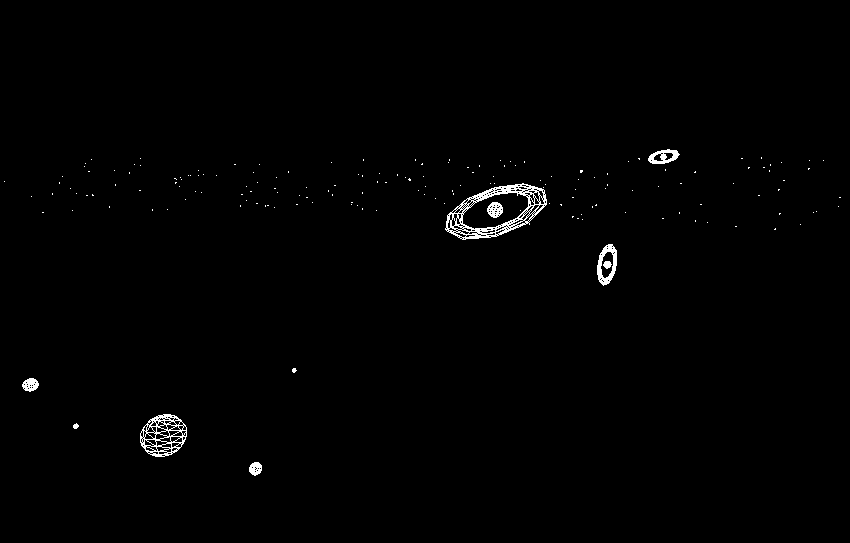
\includegraphics[width=0.9\linewidth]{res/phase2/results/SolarSystemOverview.png}
    \caption{Sistema solar com anéis e cinturas de asteróides visíveis.}
\end{figure}

Ainda existem muitas melhorias que podem ser feitas ao sistema solar, como movimento dos corpos
ou texturas.
Pretendemos implementa-las na próxima fase.

\subsection{Parametrização pelo Utilizador}

O sistema solar pode ser gerado de forma personalizada, atrvés dos seguintes parâmetros
definidos
pelo utilizador, via linha de comandos:

\begin{itemize}
    \item \texttt{sceneScale} — Escala global aplicada a toda a cena.
    \item \texttt{sunSizeFactor} — Escala atribuída ao Sol.
    \item \texttt{planetSizeFactor} — Escala definida para os planetas.
    \item \texttt{moonSizeFactor} — Escala definida para os satélites naturais.
    \item \texttt{distanceFactor} — Proporção da distância entre os diferentes corpos
celestes.
    \item \texttt{asteroidBeltDensity} — Densidade definida para as cinturas de asteróides.
    \item \texttt{ringSizeFactor} — Proporção dos anéis em relação ao planeta.
\end{itemize}

O objetivo destes parâmetros é gerar modelos do sistema solar com diferentes escalas e
proporções, para facilitar a experiência do utilizador.

\section{Extras}

\textbf{\color{red} TODO - extras}

\section{Resultados obtidos}

\textbf{\color{red} TODO - resultados}

\section{Conclusão e Trabalho Futuro}

\textbf{\color{red} TODO - conclusão}

\begingroup
\section{Bibliografia}
\renewcommand{\section}[2]{}

\begin{thebibliography}{9}
    \bibitem{exemplo}
        \href{https://youtu.be/dQw4w9WgXcQ}{Um item de exemplo na bibliografia}
\end{thebibliography}
\endgroup

\end{document}
